\documentclass[twocolumn,superscriptaddress]{revtex4-1}

%
% Preamble
%

% Fonts
\usepackage[T1]{fontenc}
\usepackage{libertine}

% Force \texttt to use Computer Modern Typewriter
\renewcommand{\ttdefault}{cmtt}
\usepackage{xspace}

% Graphics
\usepackage{graphicx}
\usepackage{float}
\usepackage{subcaption}
\usepackage[inline]{enumitem}
\usepackage{booktabs}
\usepackage[title]{appendix}
\usepackage{multirow}
\usepackage[version=4]{mhchem}
\usepackage{xcolor}

% Bibliography
\makeatletter
\renewcommand{\bibsection}{%
  \section*{\refname}%
}
\makeatother

% Hyperlinks
\usepackage{hyperref}

% Math 
\usepackage{mathtools,amsmath,amssymb}
\usepackage{braket}
\usepackage{algorithm}
\usepackage{algorithmicx}
\usepackage{algpseudocode}
\usepackage{mdframed}       % nice framed box
\usepackage{bm}

\renewcommand{\algorithmicrequire}{\textbf{Input:}}
\renewcommand{\algorithmicensure}{\textbf{Output:}}

% macros for notation
\newcommand{\abinit}{\textsc{Abinit}\xspace}
\newcommand{\atompaw}{\textsc{atompaw}\xspace}
\newcommand{\npw}{n_\mathrm{pw}}
\newcommand{\nband}{n_\mathrm{band}}
\newcommand{\nproj}{n_\mathrm{proj}}
\newcommand{\ndeg}{n_\mathrm{deg}}
\newcommand{\ecut}{E_\mathrm{cut}}
\newcommand{\xgtools}{\texttt{xgTools}\xspace}
\newcommand{\blas}{BLAS\xspace}
\newcommand{\lapack}{LAPACK\xspace}
\newcommand{\openmp}{OpenMP\xspace}
\newcommand{\gemm}{\texttt{gemm}\xspace}
\newcommand{\hegvd}{\texttt{hegvd}\xspace}
\newcommand{\nvidia}{NVIDIA\xspace}
\newcommand{\amd}{AMD\xspace}
\newcommand{\openmptarget}{OpenMP \texttt{target}\xspace}
\newcommand{\openmpoffload}{OpenMP offloading\xspace}
\newcommand{\mpi}{MPI\xspace}
\newcommand{\hip}{HIP\xspace}
\newcommand{\cublas}{cuBLAS\xspace}
\newcommand{\cufft}{cuFFT\xspace}
\newcommand{\rocblas}{rocBLAS\xspace}
\newcommand{\rocfft}{rocFFT\xspace}
\newcommand{\cusolver}{cuSOLVER\xspace}
\newcommand{\rocsolver}{rocSOLVER\xspace}
\newcommand{\rocm}{ROCm\xspace}
\newcommand{\cuda}{CUDA\xspace}
\newcommand{\cray}{Cray\xspace}
\newcommand{\llvm}{\texttt{llvm}\xspace}
\newcommand{\nvhpc}{NVHPC\xspace}
\newcommand{\topaze}{\textit{Topaze}\xspace}
\newcommand{\jeanzay}{\textit{Jean Zay}\xspace}
\newcommand{\adastra}{\textit{Adastra}\xspace}
\newcommand{\lobpcg}{LOBPCG\xspace}
\newcommand{\chebyshevfiltering}{Chebyshev filtering\xspace}
\newcommand{\alltoall}{all-to-all communication\xspace}
\newcommand{\kpoint}{$\bm{\mathsf{k}}$-point\xspace}
% end macros

% Custom colors
\definecolor{cfblue}{HTML}{005A9C}
\definecolor{capri}{rgb}{0.0, 0.75, 1.0}

%%%%%%%%%%%%%%%%%%%%%%%%%%%%%%%%%%%%%%%%%%%%%%%%%%%%%%%%%%

 
\begin{document}

\title{GPU acceleration of plane-wave density functional theory calculations in \abinit}

\author{Ioanna-Maria Lygatsika}
\thanks{Corresponding author, Present address: COMMEDIA, Laboratoire Jacques–Louis Lions, Sorbonne Universit\'e and Inria Paris, 2 rue Simone Iff, 75012
Paris, France. Email: \href{mailto:ioanna-maria.lygatsika@inria.fr}{ioanna-maria.lygatsika@inria.fr}}
\affiliation{CEA DAM-DIF, F-91297 Arpajon, France}
\affiliation{Universit\'e Paris-Saclay, CEA, LMCE, F-91680 Bruy\`eres-le-Ch\^atel, France}

\author{Marc Sarraute}
\affiliation{Alliance Service Plus, 62 rue Emile Zola, F-91200 Boulogne-Billancourt, France}

\author{Lucas Baguet}
\affiliation{CEA DAM-DIF, F-91297 Arpajon, France}
\affiliation{Universit\'e Paris-Saclay, CEA, LMCE, F-91680 Bruy\`eres-le-Ch\^atel, France}

\author{Pierre Kestener}
\affiliation{CEA DAM-DIF, F-91297 Arpajon, France}
\affiliation{Universit\'e Paris-Saclay, CEA, LiHPC, F-91680 Bruy\`eres-le-Ch\^atel, France}

\author{Marc Torrent}
\affiliation{CEA DAM-DIF, F-91297 Arpajon, France}
\affiliation{Universit\'e Paris-Saclay, CEA, LMCE, F-91680 Bruy\`eres-le-Ch\^atel, France}

\begin{abstract}

We report on the GPU port of the \abinit high-performance simulation code for plane-wave DFT calculations. Large-scale electronic structure calculations require computing the electronic wave function by solving the Kohn-Sham equations discretized over a large number of plane waves. Porting such calculations to GPU nodes relies not only on extensive usage of vendor libraries from a development perspective, but also on algorithmic revisions of the iterative diagonalization procedure in the resolution of the Kohn-Sham equations to identify GPU-efficient mathematical operations (linear algebra, FFTs) applied to the wave function distributed in memory. The present contribution discusses the \abinit implementation on multi-GPU architectures, providing detailed performance results for heterogeneous CPU-GPU nodes versus CPU nodes. Particular attention is given to comparing two diagonalization algorithms---Locally Optimal Block Preconditioned Conjugate Gradient and Chebyshev polynomial filtering---in terms of GPU efficiency.

\end{abstract}

\maketitle

\section{Introduction}

Large-scale simulations in materials science at the quantum level involve the computation of thousands of electronic states. This raises a challenge when it comes to efficiently exploiting the latest High-Performance Computing (HPC) architectures for reducing the simulation time, mainly due to the large problem size in terms of the number of states. Over the past decade, graphics processing units (GPU) have become widely available as accelerators in modern HPC systems. The advent of accelerators comes on top of an existing parallel programming landscape relying on multi-core architectures. The progressive evolution of hardware has led HPC simulation code developers to adopt new hybrid programming models for heterogeneous architectures. As GPU vendor libraries have become increasingly available, the porting task is facilitated to a great extent. Electronic structure calculations using \textit{ab initio} methods, namely Kohn-Sham Density Functional Theory (DFT) \cite{PhysRev.136.B864,PhysRev.140.A1133}, are a great candidate for GPU architectures due to the computationally expensive linear algebra operations required to calculate the electronic wave function, specifically the diagonalization of Hamiltonians over a large number of plane waves, which GPUs accelerate efficiently.

In recent years, several \textit{ab initio} codes in material science have been ported to GPU: we cite \textsc{Quantum ESPRESSO}~\cite{QE_GPU}, \textsc{Vasp} using plane-wave basis sets~\cite{https://doi.org/10.1002/jcc.23096,10.1007/978-3-319-78054-2_8,10.1007/s11227-024-06066-0}, \textsc{BigDft} using wavelet basis sets~\cite{genovese2011improvements}, \textsc{Gpaw} using real space discretization~\cite{10.1063/5.0182685}, as well as finite element codes \cite{DAS2022108473,10.1145/3295500.3357157} among others \cite{10.1063/5.0260892}. This paper concerns the widely used \abinit open-source simulation software, an international collaborative project for material science based on \textit{ab initio} methods using plane-wave basis \cite{Verstraete2025}. For several years, \abinit has utilized supercomputer architectures \cite{GAVINI2023} and regularly adapts to modern programming standards: massively parallel programming (\mpi), computing on multi-core architectures (hybrid \mpi-\openmp), and lately CPU-GPU hybridization. The present paper aims at presenting the state-of-the-art of the GPU port of \abinit towards this modernization effort.

GPU porting of \abinit dates back to 2009, with the first use of accelerators introduced through the ``recursion method'', which allows the computation of the density (and the energy) without computing any orbital. This method is only efficient at very high temperatures and is not usable for standard calculations. In 2010, plans were made to use GPUs in the ground-state calculations of \abinit, accompanied by a code analysis to identify parts that could be ported to the GPU. In 2011, the first GPU version of \abinit (v6.12) was implemented. By 2012, portability improvements were made: automatic tests were created, and the code was tested and successfully ported to \nvidia Fermi accelerators. This early GPU port was based on custom \cuda kernels, with batched FFTs (wave function not batched yet) and iterative diagonalization algorithms using MAGMA library~\cite{magma} for \nvidia only. This way of using \cuda to port \abinit to GPU was discontinued. Another earlier \nvidia GPU implementation employed the Kokkos performance portability library \cite{CARTEREDWARDS20143202} with the \cuda backend. The current GPU version of \abinit, re-implemented over the past two years from scratch, uses the \mpi-\openmp GPU offloading programming model and new low-level libraries provided by GPU vendors for executing mathematical operations \cite{torrent:tel-04812107}.

We summarize our contributions as follows:
\begin{itemize}
    \item \textit{Overview of porting strategy.} We present porting concepts focusing on specific parts of the code successfully ported to GPU: matrix-matrix multiplications, FFTs, linear algebra operations.
    \item \textit{GPU-resident wave function calculations.} The wave function is updated regularly and maintained in GPU memory. We explain how we optimized memory usage and exploited batch processing for this calculation. We provide \mpi communication theoretical estimates for two iterative diagonalization algorithms: Locally Optimal Block Preconditioned Conjugate Gradient (\lobpcg) and Chebyshev polynomial filtering. 
    \item \textit{GPU performance metrics.} We introduce metrics that allow to examine wave function calculation steps under the prism of arithmetic intensity and GPU memory bandwidth. We report an in-depth comparison of diagonalization algorithms, focusing on execution time, energy consumption and roofline models on GPUs, for assessing performance portability and comparing energy efficiency between vendors.
\end{itemize}

\section{Porting framework}\label{sec:gen_port}

This section presents the key considerations and computational design patterns at the core of \abinit{}'s GPU porting, irrespective of the programming model. We highlight the computational structure underlying wave function calculations and identify the shared characteristics of numerically intensive workloads that enabled efficient GPU porting, making our application well suited for GPU architectures. Additionally, we describe data movement concepts employed in GPU memory.

Firstly, Section~\ref{sec:batch} focuses on batch processing as key computational principle in \abinit. Section~\ref{sec:transfer} describes host-device data transfers. Section~\ref{sec:MPI_between_GPU} details the data distribution across GPUs and the MPI communication pattern between them. Lastly, Section~\ref{sec:limdims} briefly outlines the problem sizes dimensioning \textit{compute-bound}, \textit{memory-bound} and \textit{communication-bound} operations and kernels, such as large matrix operations, prior to examining them in detail in Section~\ref{sec:iterative}.

\subsection{Batch processing} \label{sec:batch}

Batch processing programming approach is crucial for the GPU port, as it determines how routines and kernels execute when computing the primary object of interest---the electronic wave function $\Psi$. Numerical solvers make use of batch processing at the level of plane waves and of electronic bands, i.e., rows and columns of $\Psi$ respectively. Throughout this document, let $N$ denote the number of plane waves and $M$ the number of electronic bands.

In essence, batch processing consists of regrouping data to operate on larger chunks instead of many smaller ones. Regrouping the data exposes coarser-grained data parallelism, so as to provide a workload better suited to exploiting the computational power of GPUs. A requirement is that the task applied to each batch must be independent for all data and able to run asynchronously, typically in the sense of the SIMD (Single Instruction, Multiple Data) programming model. The use of batch processing is crucial for limiting device memory (DRAM) traffic overhead (bytes transferred) and for improving GPU kernel throughput.

The most representative example of task on batched data is the application of the plane-wave Hamiltonian operator, that can be executed on multiple electronic bands at once instead of per band in a loop. One of the main operations underlying the application of the plane-wave Hamiltonian is fast Fourier transform (FFT). The main idea is to execute many independent FFTs asynchronously instead of relying on parallel FFT implementations. To do this, we treat the matrix $\Psi$ as a batch of column vectors and apply FFT to each column independently by a single kernel call. Porting this operation on GPU follows the batched execution illustrated in Algorithm~\ref{algo:batched_fft}, compared to a less efficient band-wise execution shown in Algorithm~\ref{algo:perband_fft}.

\begin{figure}[ht]
\centering
\scriptsize
\setlength{\arrayrulewidth}{0.3pt} % thinner lines
\setlength{\tabcolsep}{4pt}        % less horizontal padding
\begin{tabular}{|c|}
\hline
% First box
\begin{minipage}[t]{0.85\linewidth}
\begin{algorithmic}[1]
\For{$\Psi_i\in \Psi_1,\ldots,\Psi_M$}
    \State $\Psi_i \gets \text{ApplyLocalPotential}(\Psi_i)$\hfill\texttt{fftw\_plan\_dft\_3d} (\textit{CPU})
    \Statex \hfill$\rightarrow$ \texttt{xfftPlan3D} (\textit{GPU})
\EndFor
\end{algorithmic}
\captionof{algorithm}{Per-band execution.}
\label{algo:perband_fft}
\end{minipage}
\\ \hline
% Second box
\begin{minipage}[t]{0.85\linewidth}
\begin{algorithmic}[1]
\State $\Psi\gets\text{ApplyLocalPotential}(\Psi)$\hfill\texttt{fftw\_plan\_many\_dft} (\textit{CPU})
\Statex \hfill$\rightarrow$\texttt{ xfftPlanMany} (\textit{GPU}) 
\end{algorithmic}
\captionof{algorithm}{Batched bands execution.}
\label{algo:batched_fft}
\end{minipage}
\\ \hline
\end{tabular}
\caption{GPU ports of the main routines from the FFTW library \cite{frigo1998fftw} on CPU, for computing the application of the local part of Hamiltonian operator over $M$ electronic bands, followed by GPU kernels from the xFFT library, for $\text{x}=$``cu'' \cite{cufft} (\cuda API on \nvidia GPUs) or ``roc'' \cite{rocfft} (\rocm API on \amd GPUs).}
\label{fig:batched_H}
\end{figure}

The \abinit code previously implemented batch processing on CPUs for vectorized architectures within a single core~\cite{GONZE2016106, GONZE2020107042}. This optimization consisted in regrouping data into batches, that allowed to replace level-2 \blas operations by level-3 ones and FFTs to multiple vectors of plane-wave coefficients at once. The wave function is thus globally treated by blocks on CPU and the GPU port was greatly facilitated by this existing feature, especially adapted to massively parallel architectures. 

While level-3 \blas and batched 3D FFTs for treating electronic bands are optimizations also found in the CPU implementation, we mention the following new batching design particularly well suited to GPU-resident algorithms. The GPU port of \abinit goes a step further by making use of many batched kernel calls on smaller matrices \cite{dongarra_batch}. This new design is adapted to highly parallel workloads as data is stored in a configurable stride in memory, where the stride is the distance between two consecutive electronic bands. An example of mathematical operation enabling this strided batch processing is batched matrix-matrix multiplication when applied to a group of small matrices independently. The latter is a new operation only present on the GPU port and for this reason it is discussed in more detail in Section~\ref{sec:lowlevelops}. 

\subsection{Host-device memory transfers} \label{sec:transfer}

The heaviest data move between host and device happens at the wave-function level. As a consequence, it is critical to offload most wave-function-based computations to the GPU while minimizing host-device data transfers. In order to port the wave function calculation to GPU, the wave function must first be transferred to GPU. The main strategy consists in performing a single transfer of the wave function from CPU to GPU at the start of every self-consistent field (SCF) iteration for the current \kpoint of the reciprocal space. Then we avoid any intermediate transfers and keep the wave function for that \kpoint entirely on GPU memory to perform the diagonalization of a constant number of Hamiltonian applications operator, as seen in step 5 of Algorithm~\ref{algo:scf}. 

An additional host-device memory transfer is performed after treating all \kpoint{}s for the needs of computing the electronic density function from occupations and converged wave function coefficients for every \kpoint{} (see step 11 of Algorithm~\ref{algo:scf}). This involves an FFT operation on GPU.

\begin{figure}[ht]
\centering
\scriptsize
\setlength{\arrayrulewidth}{0.3pt} % thinner lines
\setlength{\tabcolsep}{4pt}        % less horizontal padding
\begin{tabular}{|c|}
\hline
\begin{minipage}[t]{0.95\linewidth}
\begin{algorithmic}[1]
\State Initialize $\Psi$. \hfill\textit{(on CPU)}
\While{self-consistent field iteration}
\For{every \kpoint{}}
\State {\color{cfblue}\textbf{Copy}} $\Psi$ for current \kpoint from CPU to GPU.\hfill\textit{(H2D)}
\State Solve $H\Psi=\Lambda S\Psi$ for current \kpoint.\hfill\textit{(solver on GPU)}
\State {\color{cfblue}\textbf{Copy}} $\Psi$ for current \kpoint from GPU to CPU.\hfill\textit{(D2H)}
\EndFor
\State Compute electronic occupations $f$ from $\Psi$.\hfill\textit{(on CPU)}
\For{every \kpoint{}}
\State {\color{cfblue}\textbf{Copy}} $\Psi$ for current \kpoint from CPU to GPU.\hfill\textit{(H2D)}
\State Accumulate electronic density from $f,\Psi$ for current \kpoint.
\Statex \hfill\textit{(FFT on GPU)}
\EndFor
\State \textbf{if} convergence met \textbf{then} exit
\EndWhile
\State \textbf{return} $\Psi$
\end{algorithmic}
\captionof{algorithm}{Self-consistent field in DFT.}
\label{algo:scf}
\end{minipage}
\\ \hline
\end{tabular}
\caption{Host-device memory transfers (H2D denoting host-to-device and D2H device-to-host) in main wave-function computation for GPU-resident diagonalization (step 5) performed iteratively within SCF outer loop. $H$ is the plane-wave Hamiltonian at current SCF iteration and $S$ the PAW overlap matrix \cite{Blochl1994}.}
\label{fig:gpu_cpu_transfer}
\end{figure}

\subsection{Communication between GPUs}\label{sec:MPI_between_GPU}

In the GPU port of \abinit, all \mpi data transfers are implemented using a GPU-aware \mpi implementation, i.e. allowing hardware-specific optimizations, and support GPU pointers. To every \kpoint, we associate a set of parallel processes. The \mpi distribution of the wave function for a given \kpoint is implemented in a 2D processor grid as follows. The matrix of column vectors---each representing the coefficients of a wave function in the plane-wave basis---is uniformly distributed across a user-defined number $p$ of \mpi processes. In \abinit, each \mpi task is associated with a single GPU (note that several \mpi tasks can share the same GPU). Two types of wave-function distributions are required, depending on the computation:
\begin{itemize}
    \item Row-distributed, suited to operations involving all columns, or electronic bands, such as linear algebra solvers, and
    \item Column-distributed, suited to the application of the Hamiltonian and FFTs since each process holds the full set of plane waves.
\end{itemize}

\begin{figure*}[ht]
    \centering
    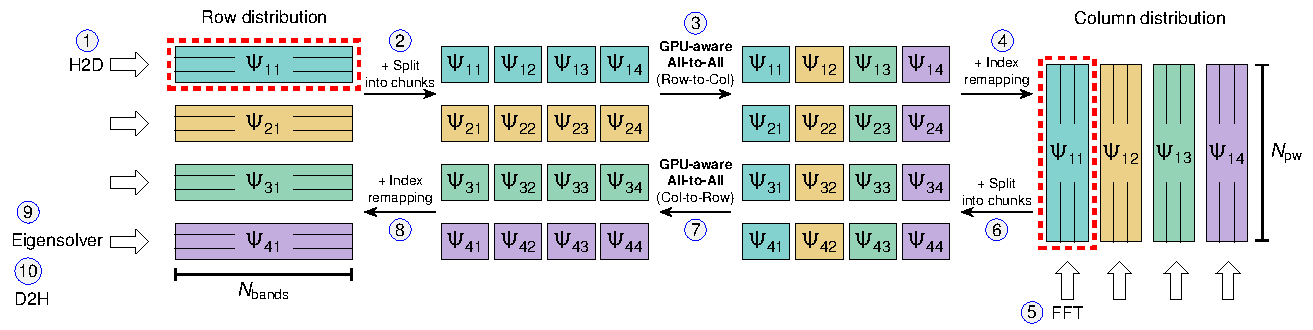
\includegraphics[width=0.9\textwidth]{Figure_1.pdf}
    \caption{Row-to-column and column-to-row \mpi transpositions of the wave function $\Psi$ distributed across $p=4$ processes. Data transfer is managed by GPU-aware MPI library. Mathematical operations (FFTs, eigensolver) are executed per block (red dashed border) in parallel. In practice, we perform all-to-all-v communication to distribute plane-wave indices as uniformly as possible during row splitting.}
    \label{fig:mem_wf}
\end{figure*}

Switching between wave-function \mpi distributions is executed by performing an all-to-all collective communication \cite{BOTTIN2008329}. The default distribution is by rows. Figure~\ref{fig:mem_wf} illustrates the \mpi transposition operation.  Host-device memory transfers are executed only before and after all-to-all communications, thus the two can be entirely decoupled when GPU-aware \mpi is enabled.

\subsection{Limiting dimensions} \label{sec:limdims}

Limiting dimensions are responsible for bottlenecks and condition scaling. These dimensions, along with mathematical operations most highly affected, are:
\begin{itemize}
    \item number of electronic bands: linear algebra operations used for orthogonalization and diagonalization procedures,
    \item number of plane waves: size of FFTs (assuming batched band execution), matrix-matrix multiplications.
\end{itemize}

Note that \kpoint treatment is highly efficient and requires minimal communication, and is therefore not a limiting dimension. Fortunately, the mathematical operations constrained by limiting dimensions are inherently GPU-friendly, suggesting strong portability potential for our code. The following section further explains how limiting dimensions affect algorithms.

\section{Iterative algorithms}\label{sec:iterative}

Iterative diagonalization is key in plane-wave DFT to compute electronic wave functions using so-called \textit{matrix-free} algorithms. The solvers for this step are the most time-consuming part of plane-wave based electronic structure calculations. In this section, we present the parallel design of available solvers in \abinit and provide theoretical estimates to model their cost, in terms of computation in FLOPS (floating point operations per second), \mpi communications (message count and communication volume) and arithmetic intensity. We then use these theoretical estimates to predict the GPU-efficient parts and bottlenecks of our solvers from an algorithmic perspective.

\subsection{Problem setup}

The Kohn-Sham equations for electronic wave functions $\psi_i$ ($i=1,\ldots,M$) read $H\psi_i = \lambda_i S\psi_i$, where $H$ is the Hamiltonian operator and $S$ the overlap operator for the $\psi_i$. $S = I$ only with norm-conserving pseudopotentials; $S \neq I$ whenever the norm constraint is relaxed, as in Projector Augmented-Wave (PAW) approach \cite{Blochl1994}. $H$ and $S$ are $N\times N$ Hermitian matrices and $\Psi=(\psi_i)_{1\leq i\leq M}$ is a $N\times M$ matrix of wave functions expressed in plane wave basis. We assume in this section that the electronic density is fixed and we are within a fixed SCF iteration, that is, in step 4 of Algorithm~\ref{algo:scf}. We look for the first smallest $M\ll N$ eigenpairs of $H$. The iterations used within the diagonalization will be referred to as \textit{inner} iterations to distinguish from SCF \textit{outer} iterations, not discussed here.

\subsection{Main computational kernels}

We describe here the core components of available iterative solvers in \abinit from a mathematical point of view, independently of their implementation.

\paragraph{Eigensolvers.} All iterative diagonalization algorithms for the Hamiltonian follow a two-step process:

\begin{enumerate}[label=(\roman*)]
\item Subspace iteration: Build a subspace by iterating on trial vector blocks, e.g., via Krylov methods, conjugate gradient (CG) residual minimization, or spectral filtering.
\item Eigenvector extraction: Diagonalize the Hamiltonian inside the subspace spanned by trial vectors to extract an approximate eigenspace using the \textit{Rayleigh–Ritz} (RR) procedure.
\end{enumerate}
The first step iteratively refines a set of trial vectors to approximate an invariant subspace, while the second step is a direct solver that yields the directions inside the invariant subspace that best approximate the actual eigenbasis. The Rayleigh-Ritz procedure is illustrated in Algorithm~\ref{fig:algo_RR}. It consists of first projecting the Hamiltonian to the trial subspace, then solving a smaller generalized eigenproblem on the subspace, finally rotating the obtained solution to recover approximated eigenvectors.

\begin{figure}[hb]
  \centering
  \scriptsize
  \setlength{\arrayrulewidth}{0.3pt} % thinner lines
  \setlength{\tabcolsep}{4pt}        % less horizontal padding
  \begin{tabular}{|c|c|}
  \hline
  % First box
  \begin{minipage}[t]{0.45\linewidth}
  \begin{algorithmic}
        \Require{Matrices $H,S$, trial vectors $\Psi$.}
        \Ensure{Solution of $(\Lambda,\Psi)$.}
        \State $H_{\Psi} =\Psi^\top H\Psi$
        \State $S_{\Psi} = \Psi^\top S\Psi$
        \State $H_{\Psi}X = \Lambda S_{\Psi}X$ \hfill \hegvd
        \State $\Psi\gets X^\top \Psi$
        \vspace{7ex}
      \end{algorithmic}
  \captionof{algorithm}{Standard.}
  \label{fig:algo_RR}
  \end{minipage}
  &
  % Second box
  \begin{minipage}[t]{0.45\linewidth}
  \begin{algorithmic}
        \Require{Trial vectors $\Psi, \texttt{H}\Psi,\texttt{S}\Psi$.}
        \Ensure{Solution $(\Lambda,\Psi),\texttt{H}\Psi,\texttt{S}\Psi$.}
        \State $H_{\Psi} =\Psi^\top (\texttt{H}\Psi)$ \hfill \gemm
        \State $S_{\Psi} = \Psi^\top (\texttt{S}\Psi)$ \hfill \gemm
        \State $H_{\Psi}X = \Lambda S_{\Psi}X$ \hfill \hegvd
        \State $\Psi\gets X^\top \Psi$ \hfill \gemm
        \State $\texttt{H}\Psi\gets X^\top (\texttt{H}\Psi)$ \hfill \gemm
        \State $\texttt{S}\Psi\gets X^\top (\texttt{S}\Psi)$ \hfill \gemm
  \end{algorithmic}
   \captionof{algorithm}{Matrix-free.}
   \label{fig:algo_dft}
  \end{minipage}
   \\ \hline
  \end{tabular}
  \caption{Rayleigh-Ritz (RR) procedure for solving the generalized eigenvalue problem $H\Psi=\Lambda S\Psi$. Here $\texttt{H}\Psi$ and $\texttt{S}\Psi$ denote the matrices obtained after matrix-free application of operators $H$ and $S$ to $\Psi$. \abinit implements the matrix-free version.}
\end{figure}

\paragraph{Matrix-free application of the Hamiltonian.}

In plane-wave basis, applying the Hamiltonian operator to an arbitrary coefficient vector involves FFTs and local multiplications. \abinit implements a \textit{matrix-free} application of the plane-wave Hamiltonian. Matrix-free algorithms save memory by applying the Hamiltonian to a wave function (or any input column vector) without explicit allocation of any memory for storing the Hamiltonian matrix. Matrix-free algorithms are well-suited to plane-wave DFT because the number of wanted eigenpairs is much smaller than the number of plane-wave basis elements (typically few percents). For instance, for medium to large systems the order of magnitude is typically 10k–30k sought eigenpairs for 100k–1M plane waves. Moreover, the plane-wave Hamiltonian is dense, so explicit storage would scale quadratically with the number of plane waves. Matrix-free methods reduce memory requirements to linear scaling in the number of plane waves. The matrix-free version of the Rayleigh-Ritz procedure implemeted in \abinit is illustrated in Algorithm~\ref{fig:algo_dft}.

\paragraph{Subspace iteration.}

\abinit implements two main classes of algorithms for constructing the trial subspace, using two different approaches. The first one is \textit{vector-oriented} and partitions the wave function into blocks of vectors to apply a block resolution, such as the Locally Optimal Block Preconditioned Conjugate Gradient (\lobpcg) \cite{BOTTIN2008329}, while the second one is \textit{spectrum-oriented} and filters the eigenvalue spectrum using analytical properties of polynomials to amplify wanted spectral intervals, such as \chebyshevfiltering \cite{LEVITT201598} (using Chebyshev polynomials). All steps of these two families of algorithms are offloaded to GPUs allowing to keep the wave function in GPU-resident memory. Figure~\ref{fig:batched_filter} illustrates the block structure used by the two classes of algorithms when applying elementary operations on the wave function. Note that polynomial filtering eliminates inter-block dependencies, contrary to vector-oriented \lobpcg that includes inter-block dependence when orthogonalization with respect to previous blocks. Finally, a global solver call based on the Rayleigh-Ritz procedure is common in both methods.

\begin{figure}[ht]
\centering
\scriptsize
\setlength{\arrayrulewidth}{0.3pt} % thinner lines
\setlength{\tabcolsep}{4pt}        % less horizontal padding
\begin{tabular}{|c|}
\hline
% First box
\begin{minipage}[t]{0.85\linewidth}
\begin{algorithmic}
\For{$n=0,\ldots,k$}
    \For{$\Psi_i \in \Psi_1,\ldots,\Psi_b$}
        \State $\Psi_i \gets \text{RefineSubspaceBlock}(\Psi_1,\ldots,\Psi_i)$\hfill\textit{(H app.+ortho+CG)}
        \State $\Psi_i\gets\text{ExtractEigenvectorsBlock}(\Psi_i)$\hfill\textit{(block solver=RR)}
    \EndFor
\EndFor
\State $\Psi\gets\text{ExtractEigenvectors}(\Psi)$\hfill\textit{(global solver=RR)}
\end{algorithmic}
\captionof{algorithm}{\lobpcg with $b$ blocks and $k$ line minimizations.}
\end{minipage}
\\ \hline
% Second box
\begin{minipage}[t]{0.85\linewidth}
\begin{algorithmic}
\For{$n=0,\ldots,k$}
    \State $\Psi \gets \text{SpectralFiltering}(\Psi)$\hfill\textit{(H app.)}
\EndFor
\State $\Psi\gets\text{ExtractEigenvectors}(\Psi)$\hfill\textit{(global solver=RR)}
\end{algorithmic}
\captionof{algorithm}{Spectral polynomial filtering of degree $k$.}
\end{minipage}
\\ \hline
\end{tabular}
\caption{Schematic description of GPU-ported eigensolvers used to solve $H\Psi=\Lambda S\Psi$. Note that elementary core components---Hamiltonian application (H app.), conjugate gradient (CG), Rayleigh-Ritz (RR)---are common to both types of algorithms, but applied to different subspaces.}
\label{fig:batched_filter}
\end{figure}

\subsection{Parallel implementation design}\label{sec:paral_design}
We focus on the parallel implementation of iterative solvers based on the main computational kernels. These operations and their respective notation are (where $n$ and $m$ denote arbitrary integers): 
\begin{itemize}
    \item $S$-orthogonalization of $m$ bands expressed in $n$ plane-wave coefficients, performed by the matrix-free routine $\texttt{S-Ortho}(n,m)$, 
    \item Rayleigh-Ritz procedure to extract $m$ eigenvectors expressed in $n$ plane-wave coefficients, performed by the matrix-free routine $\texttt{RR}(n,m)$ given by Algorithm~\ref{fig:algo_dft},
    \item Application of the Hamiltonian operator $H$ (and of the PAW overlap matrix $S$) to $m$ vectors expressed in $n$ plane-wave coefficients, performed by the matrix-free routine $\texttt{HX}(n,m)$ (and by $\texttt{HX\_SX}(n,m)$),
    \item Application of the inverse overlap operator $S$ to $m$ vectors expressed in $n$ plane-wave coefficients, using a Woodburry formulation, as explained in~\cite{LEVITT201598}, performed by the matrix-free routine $\texttt{Sinv}(n,m)$.
\end{itemize}

From now on, if $p$ is the number of parallel processes, let us define $m_p=M/p$ and $n_p=N/p$. Figure~\ref{fig:parallel_algo_bis} shows the parallel diagonalization algorithms. The Chebyshev polynomial spectrum filtering algorithm employs an auxiliary kernel to efficiently compute the Hamiltonian polynomial applied to wave functions via a recurrence relation. It involves operations of the form $X\gets aX + Y$, for $X$ and $Y$ of size $n\times m$, performed by the routine $\texttt{axpy}(n,m)$ of level-1 BLAS. Parallel processes communicate only at the end of the subspace iteration of length $k$. Note that the loop over the number of blocks as well as the loop over the number of inner iterations are intrinsically sequential. 

\begin{figure}[ht]
\centering
\scriptsize
\setlength{\arrayrulewidth}{0.3pt} % thinner lines
\setlength{\tabcolsep}{4pt}        % less horizontal padding
\begin{tabular}{|c|c|}
\hline
% First box
\begin{minipage}[t]{0.52\linewidth}
\begin{algorithmic}
\For{$n=0,\ldots,k$}
    \For{$\Psi_i \in \Psi_1,\ldots,\Psi_b$}
        \If{$b>1$}
            \State $\Psi_i\gets\texttt{S-Ortho}(n_p,M/b)$
        \EndIf
        \State {\color{cfblue}\textbf{MPI}} transpose Row-to-Column.
        \State $\texttt{H}\Psi_i,\texttt{S}\Psi_i \gets \texttt{HX\_SX}(N,m_p/b)$
        \State {\color{cfblue}\textbf{MPI}} transpose Column-to-Row.
        \State $\Psi_i\gets \texttt{S-Ortho}(n_p,M/b)$
        \State $\Psi_i,\texttt{H}\Psi_i,\texttt{S}\Psi_i\gets\texttt{RR}(n_p,M/b)$
    \EndFor
\EndFor
\State $\Psi,\texttt{H}\Psi,\texttt{S}\Psi \gets \texttt{S-Ortho}(n_p,M)$
\State $\Psi,\texttt{H}\Psi,\texttt{S}\Psi\gets\texttt{RR}(n_p,M)$
\end{algorithmic}
\captionof{algorithm}{\lobpcg.}
\end{minipage}
&
% Second box
\begin{minipage}[t]{0.42\linewidth}
\begin{algorithmic}
\State {\color{cfblue}\textbf{MPI}} transpose Row-to-Column.
\State $\texttt{H}\Psi,\texttt{S}\Psi \gets \texttt{HX\_SX}(N,m_p)$ 
\For{$n=0,\ldots,k$}
    \State $\texttt{H}\Psi \gets \texttt{HX}(N,m_p)$
    \State $\texttt{S}^{-1}\texttt{H}\Psi\gets\texttt{Sinv}(N,m_p)$
    \State $\Psi \gets \texttt{axpy}(N,m_p)$
\EndFor
\State $\texttt{H}\Psi,\texttt{S}\Psi \gets \texttt{HX\_SX}(N,m_p)$
\State {\color{cfblue}\textbf{MPI}} transpose Column-to-Row.
\State $\Psi,\texttt{H}\Psi,\texttt{S}\Psi\gets\texttt{RR}(n_p,M)$
\vspace{6ex}
\end{algorithmic}
\captionof{algorithm}{\chebyshevfiltering of degree $k$.}
\label{alg:chebfi_k}
\end{minipage}
\\ \hline
\end{tabular}
\caption{Parallel matrix-free subspace iteration algorithms for computing the wave function $\Psi$ described at the level of GPU kernels, with $k$ inner iterations. While LOBPCG (left) uses $b$ blocks, for spectral filtering (right), we consider one block only.}
\label{fig:parallel_algo_bis}
\end{figure}

The main difference between the algorithms is that \lobpcg{} makes $bk$ calls to $(M/b)$-sized Rayleigh-Ritz procedure plus a global one, whereas \chebyshevfiltering{} makes only a global one. Therefore, \lobpcg{} makes intensive use of the Rayleigh-Ritz procedure by calling it within each subspace iteration. Notably, as we demonstrate in the following, the Rayleigh-Ritz procedure scales poorly with respect to the number of bands and does not fully benefit from efficient parallelization.

\subsection{Floating-point operation count}\label{sec:flop_count}

To quantify the computational cost of each algorithm, we estimate the floating-point operation (FLOP) count using the following theoretical models. We assume that $k$ is the maximal number of inner iterations (gradient descent or polynomial filtering degree) and $b$ is the number of blocks in \lobpcg algorithm. Let $N_{\text{projs}}$ be the number of projectors involved in the overlap operator. The steps of diagonalization algorithms, as appearing in Figure~\ref{fig:parallel_algo_bis}, admit the following theoretical cost estimates. Let $m$ be an arbitrary number of bands. The routine $\texttt{RR}(n_p,m)$ approximately has a cost of $O(m^3+n_pm^2)$ FLOP (\gemm and \hegvd dense \lapack solver for the problem on a subspace of dimension $m$) \cite{doi:10.1137/070688778}. The routine $\texttt{S-Ortho}(n_p,m)$ is also dominated by cubic scaling with respect to $m$, as its implementation involves the multiplication $X^\top (\texttt{S}X)$ (\gemm routine), the Cholesky factorization of a Hermitian positive-definite matrix (\texttt{potrf} routine) and the triangular matrix solver (\texttt{trsm} routine). The routine $\texttt{HX}(N,1)$ has $O(N\log N+N_{\text{projs}}N)$ FLOP due to FFT \cite{LEVITT201598,d3ea2d52-5ab2-3128-8b80-efb85267295d}. Then $\texttt{HX}(N,m)$ has $m$ times the cost of $\texttt{HX}(N,1)$ due to batching over bands. Finally, according to \cite{LEVITT201598}, the iterative algorithm used to apply $S^{-1}$ has a cost of $O(N_{\text{projs}}^2)\ll O(N_{\text{projs}}N)$, so the total cost of $\texttt{Sinv}(N,1)$ applied on one band is $O(N_{\text{projs}}N)$.

Now, using parallelization, the cubic scaling of Rayleigh-Ritz and of orthogonalization is not affected when parallelizing over plane waves. On the other hand, by parallelizing the Hamiltonian and the $S,S^{-1}$ applications over bands, we gain a factor $1/p$ when using $p$ parallel processes. Additionally note that multithreading within a single MPI task performs poorely for the eigensolver (\texttt{hegvd}) and the Cholesky factorization (\texttt{potrf}).

Overall, the Rayleigh-Ritz procedure and $S$-orthogonalization exhibit cubic scaling with the number of bands, while the Hamiltonian application and $S$-inversion scale linearly with the number of bands. This theoretical estimate reveals that the final Rayleigh-Ritz step scales poorly in both methods and is expected to represent a computational bottleneck for systems with a large number of bands. Thus, the number of bands emerges as a limiting dimension for these operations.

\subsection{\mpi communications}

This discussion is independent of the presence of a GPU and focuses only on comparing \lobpcg and \chebyshevfiltering, all else being equal. We will examine the data transfers described in Figure~\ref{fig:parallel_algo_bis} in order to obtain a comparative estimate of the communication costs. The \mpi communication cost, in terms of latency and bandwidth usage, can be estimated using the cost model ``$\alpha+\mathsf n\beta$''~\cite{doi:10.1177/1094342005051521}, where $\alpha$ is the latency (s) (independent of the message size), $\beta$ is the inverse bandwidth and $\mathsf n$ the message size. To quantify this further, we theoretically estimate both the number of messages and communication volume for each algorithm. In \lobpcg, the \alltoall from row distribution to column distribution involves $p$ processes that send $n_p$ rows and $M/b$ columns, while the inverse operation sends $N$ rows and $m_p/b$ columns. This operation is performed $k$ times per block. With double-precision complex buffers, the message size is $16NM/(pb)$ bytes. In \chebyshevfiltering, with no blocks, the message size is $16NM/p$ bytes. In \lobpcg, back and forth MPI transpositions repeat $k$ times per CG iteration per block, whereas in \chebyshevfiltering it occurs only once. The latency, proportional to the number of communications, is then $kb$ times higher in \lobpcg than \chebyshevfiltering. Table~\ref{tab:mpi_comms} summarizes the communication costs.

This theoretical estimate shows that communication latency in \lobpcg scales linearly with the total number of blocks; thus, we expect \lobpcg to suffer from communication overhead when dealing with large systems or a larger number of blocks. It is important to keep in mind that \mpi communications are performed between GPUs if GPU-aware MPI is supported.

\begin{table}[H]
    \centering
    \begin{tabular}{l|r|r}\toprule
                                 & \texttt{\lobpcg}$(N,M,b,k)$   & \texttt{ChebFi}$(N,M,k)$ \\ \midrule
          Latency cost           &   $4kb\alpha$    &  $4\alpha$   \\
          Bandwidth cost         &   $16NM/(pb)\beta$          &  $16NM/p\beta$   \\ \bottomrule
    \end{tabular}
    \caption{Theoretical estimates of the communication costs (message size and volume) for the \lobpcg and \chebyshevfiltering (abbreviated as \texttt{ChebFi}) parallel algorithms, with $p$ parallel processes. Note there are 4 transpositions per Hamiltonian application: $\Psi$ (forward), $\Psi$ (backward), $H\Psi$ (backward), $S\Psi$ (backward).}
    \label{tab:mpi_comms}
\end{table}

\subsection{Arithmetic intensity}\label{par:arithm_intensity}

The arithmetic intensity $I$ is defined as the ratio of computational work $W$ to total memory traffic (number of read/write requests $\times$ bytes per request) $Q$: 
$$I = \frac{W}{Q}.$$
The work is measured in FLOP. Memory traffic represents the total number of bytes transferred during read/write requests to DRAM, on a single \mpi process during GPU kernels execution. Here, we aim to estimate the arithmetic intensity for kernels between two consecutive MPI communications.

Our goal is to design algorithms that maximize arithmetic intensity per \mpi process. The parallel \lobpcg and \chebyshevfiltering algorithms handle \mpi GPU-to-GPU communications differently for a fixed number $k$ of inner iterations during the subspace iteration step. Indeed, \lobpcg applies the Hamiltonian $k$ times per block (i.e., ``$k\,\times\,$Comm.--$H$ application--Comm.'' per block), resulting in a total of $4kb$ \alltoall operations. In contrast, \chebyshevfiltering only 4 global \alltoall operations in total (i.e., ``Comm.--$H^k$ application--Comm.''). Intuitively, \chebyshevfiltering maximizes arithmetic intensity by applying the Hamiltonian $k$ times more per \mpi data transposition than \lobpcg.

Indeed, an estimate of the arithmetic intensity of the GPU kernels involved in Hamiltonian applications, for a single data movement, is
\begin{align*}
    I(\text{\lobpcg-}\texttt{HX}) &= \frac{\text{FLOP}(\texttt{HX}(N,m_p/b))}{Q/b},\\
    I(\text{\chebyshevfiltering-}\texttt{HX}) &= \frac{k\times\text{FLOP}(\texttt{HX}(N,m_p))}{Q},
\end{align*}
where $Q$ is the byte count for storing a complex wave function in column-distribution of size $N\times m_p$ on the GPU in double precision, yielding $Q=16Nm_p$ bytes of input and output memory buffers. Since the Hamiltonian application is parallel in the number of bands, $\text{FLOP}(\texttt{HX}(N,m_p/b))=\text{FLOP}(\texttt{HX}(N,m_p))/b$ and finally $I(\text{\chebyshevfiltering-}\texttt{HX}) = k I(\text{LOBPCG-}\texttt{HX})$. This shows that \chebyshevfiltering maximizes the arithmetic intensity of the Hamiltonian application operation, which is well suited for GPUs thanks to its batched execution.

\section{Methods and programming models}\label{sec:methods}

This section presents specific strategies used for offloading computationally expensive parts of the code on GPUs. More details on how low-level GPU libraries communicate with the \abinit code are provided. Basically we use the following hierarchy of operations from a development view-point:
\begin{enumerate}
    \item \textit{Directive-based programming}. The\textit{} way data transfers between host and device are executed, the way we interface with GPU libraries at a programming level.
    \item \textit{Low-level operations}. Interfaces strictly connected to vendor libraries. Wrappers to libraries. Mathematical operations (matrix-matrix multiplications, FFTs, eigensolvers) are mapped to GPU libraries.
    \item \textit{Abstraction layer}. Implements data-structures adapted to the commonly used objects in \abinit, namely the wave-function. The architecture is defined using a keyword and for every architecture there is a wrapper to its implementation. Boolean options are used to control if an operation is executed on GPU or CPU.
\end{enumerate}

\subsection{\openmpoffload}

We employ the \openmpoffload programming model for GPU acceleration, using directives introduced in \openmp API version 5.0~\cite{OpenMP5.0}. \openmp handles device workload distribution, memory management and host-device data transfers via \texttt{target} directives,  with execution controlled by the
\texttt{OMP\_TARGET\_OFFLOAD} environment variable.

Computations are performed on the device within an \openmptarget region. We selected this programming model for \begin{enumerate*}[label=(\roman*)]
\item its directive-based simplicity, which facilitates porting with minimal code rewriting; \item its excellent portability across platforms; \item its limited compilation dependencies; and \item its simplified memory management, which allows allocations and frees to be handled directly in Fortran. \end{enumerate*} Together, these aspects enhance the code's readability and maintainability over time. We systematically apply the \texttt{COLLAPSE} directive for batch loop processing, enabling straightforward GPU persistent memory management. The model is also vendor-agnostic; we validated \openmptarget with \cuda and \nvhpc compiler on \nvidia GPUs (A100, H100, H200) and with \rocm and \cray compiler on \amd GPUs (MI250, MI300). We validated unified memory usage on NVIDIA GH100 and GH200, which is greatly simplified in the \openmptarget paradigm. 

\subsection{Low-level operations}\label{sec:lowlevelops}

This section summarizes the GPU implementation of elementary low-level operations. Our current approach primarily employs vendor libraries for maximum portability, avoiding custom GPU kernels. We rely on backend libraries from \cuda Toolkit \cite{cuda_manual} for \nvidia GPUs, and \rocm \cite{rocm_manual} for \amd GPUs. Calls to these vendor library functions are encapsulated in wrappers, making them transparent to the overlying software layer. 

Firstly, batching is employed to compute the FFT of multiple wave functions stored in an array through a single call, instead of applying the FFT iteratively to individual vectors. The plane-wave cut-off energy $E_{\text{cut}}$ determines the grid size, and consequently the size of the FFT, while the number of bands treated per MPI task determines the number of FFTs, consequently the batch size. This process is used when computing the local part of the Hamiltonian operator. Since this operation involves all plane waves, the data must first be rearranged into the specific layout described in section ~\ref{sec:MPI_between_GPU}. The vendor libraries \cufft \cite{cufft} and \rocfft \cite{rocfft} are then used in a batched and optimized mode to maximize reuse of precomputed data whenever possible.

Secondly, we specifically address matrix-matrix multiplications (i.e. \gemm operations) and associated routines critical for GPU-accelerated Hamiltonian. This requires replacing Fortran \blas \gemm calls with equivalents from \cublas \cite{cublas} and \rocblas \cite{rocblas}. Notably, the matrix-free plane-wave Hamiltonian application leverages level-3 \blas operations, as applications to different bands are independent—favoring matrix-matrix over matrix-vector multiplications.

Thirdly, for solvers, we employ \cusolver \cite{cusolver} and \rocsolver \cite{rocsolver} to tackle the generalized eigenvalue problem within the Rayleigh-Ritz procedure, complemented by the ELPA library~\cite{marek2014elpa} for direct eigensolvers of Hermitian matrices. This computational step proves critical, as the Rayleigh-Ritz procedure represents a major bottleneck (see Section~\ref{sec:flop_count}). Consequently, the performance of the \lapack routine \hegvd—which varies significantly across implementations—plays a pivotal role.


Finally, an explicit code refactoring enables batched kernel execution on GPUs for applying the non-local operator, expressed as $V_{\text{NL}}=\sum_{R,i,j}{\ket{p^R_i}D^R_{ij}\bra{p^R_j}}$, where the $\ket{p^R_i}$ are projectors depending on atom $R$ and local basis index $1\leq i\leq n^R_{lmn}$. Ultimately,  application requires matrix-matrix multiplications involving $P=\braket{g|p^R_i}$ (projectors in the plane-wave basis), $C_{\text{proj}}=\braket{p^R_i|\Psi}$ (projected wave functions), and $D^R_{ij}$. Since the local basis size $n^R_{lmn}$ varies by atom type, batching these matrix-matrix multiplications requires subtleties. This was addressed by refactoring the code: loops were reordered to process atomic types sequentially first, while grouping wave functions into batches. The \texttt{gemmBatchedStrided} kernel, available in \cublas and \rocblas, efficiently computes groups of matrix-matrix products on the GPU. Refactoring additionally involved transforming some function calls that previously passed Fortran array slices. Avoiding slices improves control over memory layout and exposes greater data parallelism.

\subsection{Abstraction layer}\label{sec:abstraction}

An abstraction layer enables algorithms to interface with low-level operations from a software development perspective, as illustrated in Figure~\ref{fig:xgtools}.

\begin{figure}[hb]
    \centering
    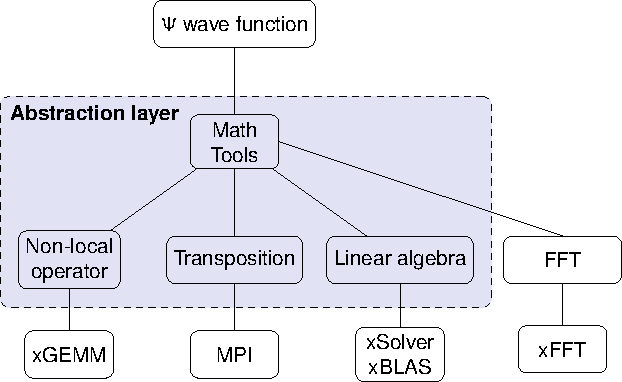
\includegraphics[width=0.95\linewidth]{Figure_2.pdf}
    \caption{Hierarchy from the high-level wave function to the low-level GPU libraries (x=``cu'', ``roc'') linked through the \abinit abstraction layer. FFT and non-local operator will be included in the abstraction layer in a future work.}
    \label{fig:xgtools}
\end{figure}

This abstraction layer provides Fortran types offering a unified, high-level interface for handling distributed matrices and vectors, performing algebraic operations, and solving generalized eigenvalue problems. These types operate on blocks of row (or column) vectors forming contiguous memory batches, with a data structure compatible with GPU architectures and support for CPU/GPU memory pointers. Designed for clarity and simplicity—especially for \abinit developers—the interface hides the underlying complexity and diversity of algebraic structures used in wave-function manipulations across linear algebra libraries.
The abstraction layer facilitates easy extension by users through additional functionalities. The \textit{Tools} framework supports matrix-free Hamiltonian applications by manipulating objects $X$ (the wave function) and $AX$ (its application under operator $A$), without needing explicit knowledge of the matrix $A$. The module manages all memory allocations/deallocations of workspaces  needed in diagonalization algorithms.

The abstraction layer also provides an interface between wave functions and \mpi routines. It enables efficient, transparent conversions between different wave function representations and their \mpi distributions (see Section~\ref{sec:MPI_between_GPU}), while managing contiguous memory layouts. All required communications are handled transparently—hidden from developers via simple routine options—supporting both row and column distributions. Sub-distributions via sub-communicators are straightforward to implement, facilitating additional parallelism across matrix blocks when needed.

The abstraction layer enables efficient execution of linear algebra operations while seamlessly interfacing with \blas and \lapack implementations for dense complex-valued matrices.

\section{Performance}\label{sec:perfs}

In this section, we present performance benchmarks and numerical results for the \abinit GPU port, focusing on acceleration and energy efficiency across \nvidia and \amd GPUs. We also discuss GPU memory usage, kernel arithmetic intensity, custom metrics, and roofline models, with particular emphasis on comparing \lobpcg and \chebyshevfiltering algorithms in inner subspace iterations their relative performance.
Computer specifications are detailed in Appendix~\ref{sec:gpu_specifs}. Systems from Table~\ref{tab:gpu_specifs} are abbreviated as \adastra (CINES), \jeanzay (IDRIS), and \topaze (CCRT).

\subsection{Test cases}

We used two distinct test cases. \textit{Converged-SCF} benchmarks (Section\ref{sec:multiple_gpu}) were obtained from converged calculations of a solid-liquid titanium interface with 255 atoms, 4096 electronic bands, PAW pseudopotentials, a cutoff energy of 20 Ha, and 1 \kpoint. The number of self-consistent iterations was fixed. These tests ran on \topaze (CCRT) and \adastra (CINES) using \abinit version 10.1 compiled with \nvhpc compiler on \nvidia and \cray compiler on \amd.

\textit{Single-step} benchmarks (Sections~\ref{sec:per_gpu_diago} and~\ref{sec:per_gpu_si}) used a second test case with constant-Hamiltonian calculations (single SCF iteration): \ce{Ga2O3} with 320 atoms and 1536 electronic bands, PAW pseudopotentials, a cutoff energy of 20 Ha, and 1 \kpoint. These tests were performed on \topaze (CCRT) using \abinit version 10.4.5 compiled with \nvhpc on \nvidia GPUs, along with Nsight Compute 2025.3~\cite{nvidia_nsight_compute} for detailed profiling.

\subsection{Results on multiple GPU nodes}\label{sec:multiple_gpu}

Using \textit{converged-SCF} test case, we compare GPU-accelerated performance and energy consumption between \texttt{n} CPU-only nodes and \texttt{n} CPU-GPU nodes---a true ``node-to-node'' comparison---for \texttt{n} ranging from 1 to 8. Each CPU-only node is directly benchmarked against one hybrid CPU-GPU node in terms of execution time and energy consumption.

\begin{figure*}[ht]
    \centering
    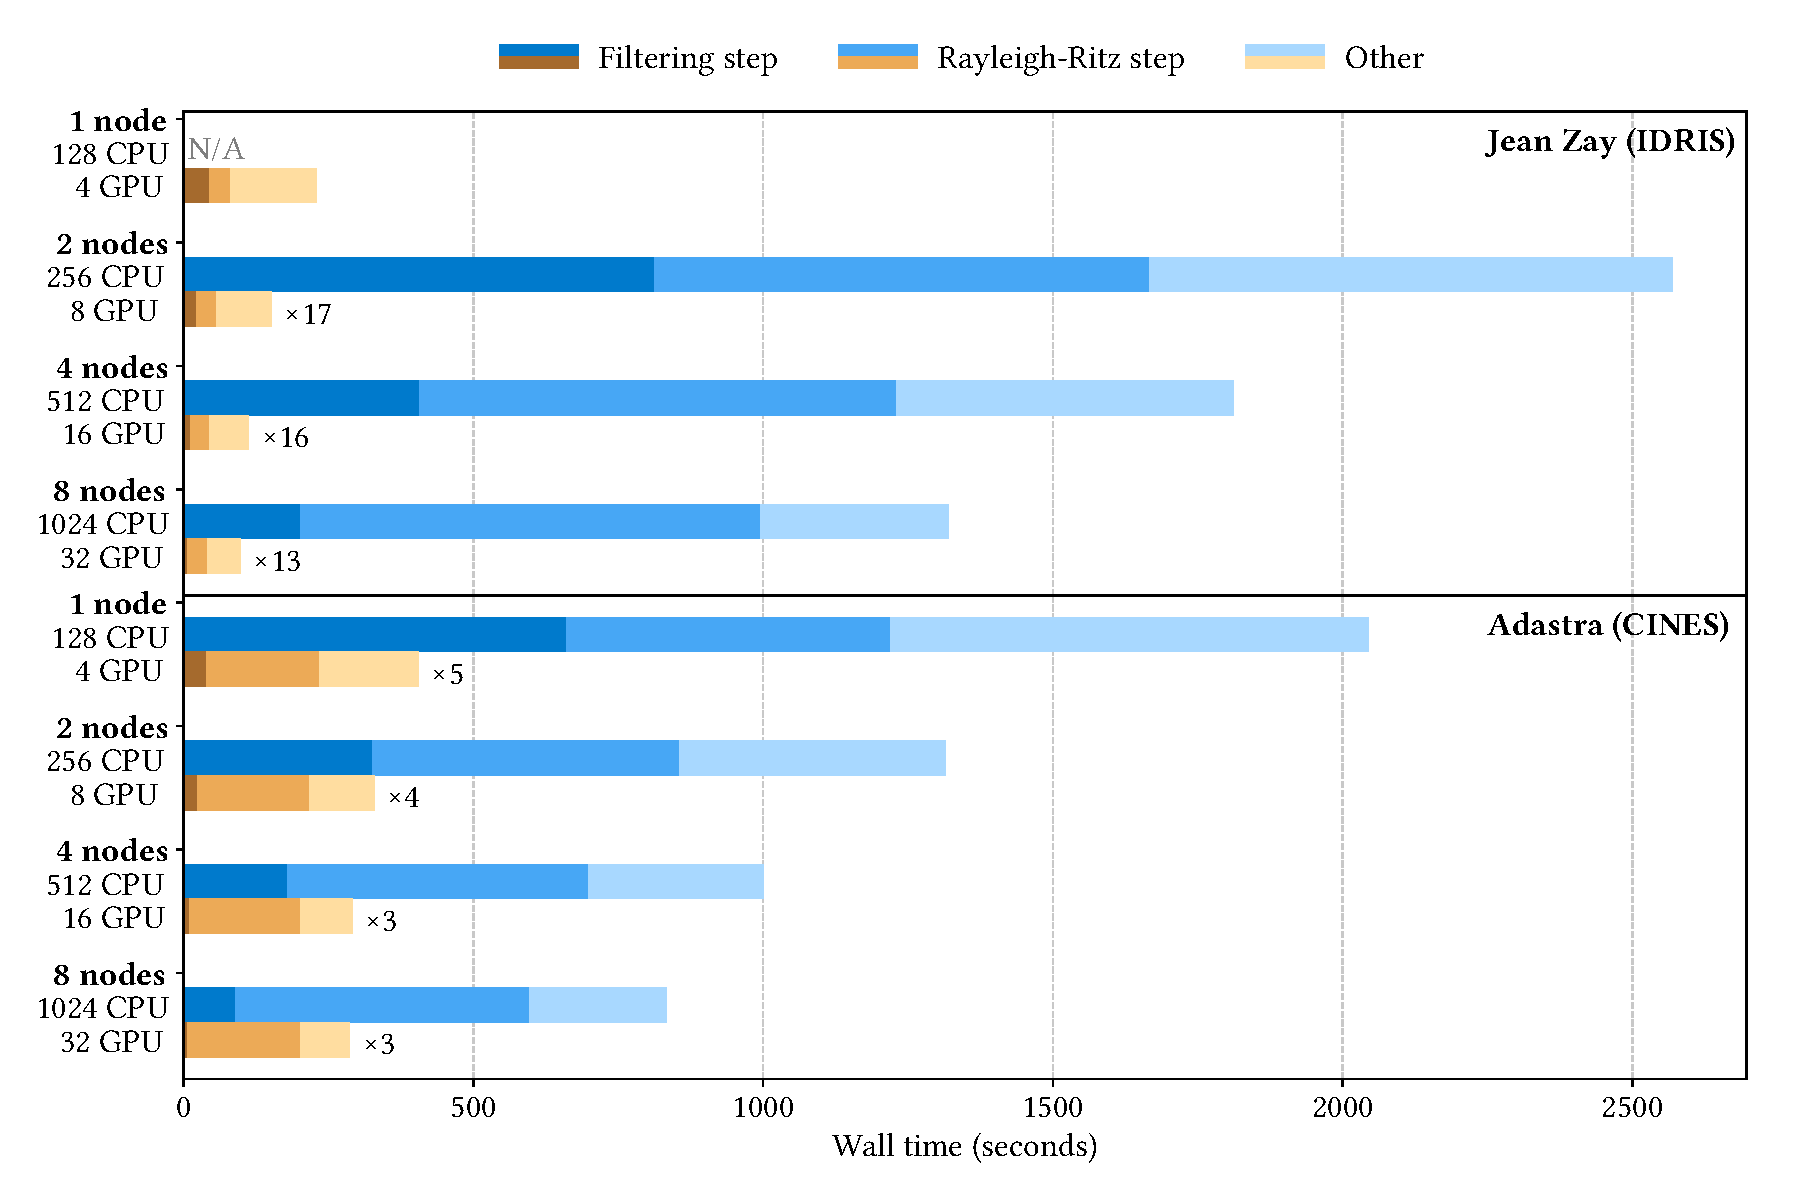
\includegraphics[width=0.8\linewidth]{Figure_3.pdf}
    \caption{Execution time and GPU speedup for \chebyshevfiltering on a 255-atom Ti system (4096 electronic bands) over 10 SCF iterations. ``Filtering step'' includes operations between \mpi transpositions in Algorithm~\ref{alg:chebfi_k}; ``Rayleigh-Ritz step'' covers subspace diagonalization; ``Other'' encompasses remaining calculations including \mpi communications. Performance comparison between \topaze (TGCC) with \nvidia GPUs (NVHPC v23.11, CUDA v12.3) and \adastra (CINES) with \amd GPUs (Cray CPE v23.12, ROCm v5.7.1).} 
    \label{fig:prel}
\end{figure*}

Figure~\ref{fig:prel} illustrates GPU speedup for \chebyshevfiltering. \nvidia GPUs consistently deliver higher speedup factors than \amd GPUs. The Rayleigh-Ritz step dominates execution time and exhibits lower acceleration than the filtering step, which becomes negligible with GPU acceleration. The Rayleigh-Ritz step proves particularly poorly suited to \amd GPUs.
Closer inspection of per-step timings reveals that the Rayleigh-Ritz portion increases with node count. Overall, filtering benefits substantially from acceleration, while Rayleigh-Ritz improves more modestly, particularly on \amd architecture. This is related to the performance of the \hegvd routine called during the Rayleigh-Ritz step. We respectively used \cusolver v12.3 on \nvidia GPUs and \rocsolver v5.7.1 on \amd GPUs. Since our performance measurements were conducted, the \rocm implementation of \hegvd has reportedly been improved in subsequent versions \cite{rocsolver_rocm642}. On \nvidia speedup is excellent: 2 GPU nodes outperform 8 CPU nodes, enabling substantial resource savings.

Figure~\ref{fig:prel} also reveals insights into strong scaling. GPU scaling efficiency lags behind CPU performance as node count grows, consistent with \textit{Amdahl’s law}. Notably, the Rayleigh-Ritz step shows no acceleration with additional GPU nodes. In practice, thanks to this limited scalability, fewer GPUs are needed compared to CPU-only scaling.

\begin{figure}[ht]
    \centering
    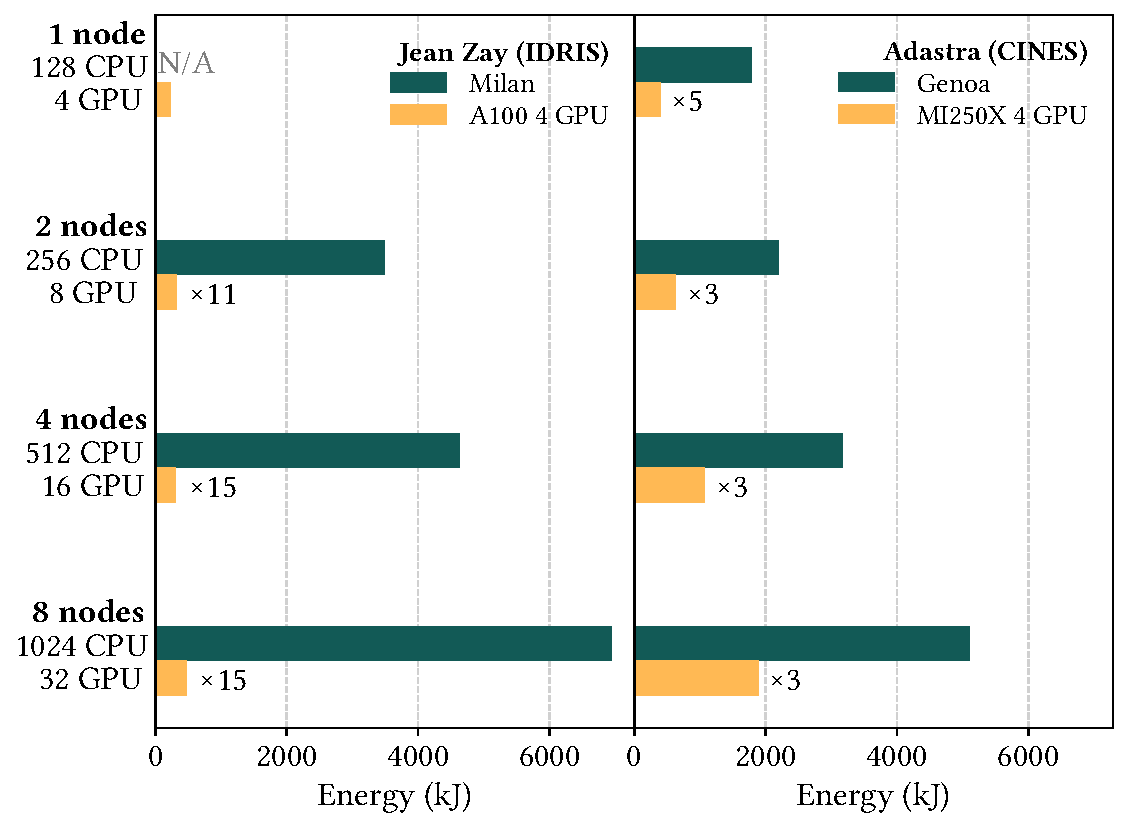
\includegraphics[width=\linewidth]{Figure_4.pdf}
    \caption{Energy consumption and savings for \chebyshevfiltering on a 255-atom Ti system (4096 electronic bands). Energy saving factors compare \topaze (CCRT, \nvidia GPUs) versus \adastra (CINES, \amd GPUs), with the same compiler and library versions as in Fig.~\ref{fig:prel}. Energy measurements are provided directly by the supercomputers and may differ between the two systems. Therefore, comparing only the energy saving factor is meaningful.} 
    \label{fig:energy}
\end{figure}

To measure energy consumption, we used vendor-provided counters and tools, executed on the same hybrid nodes, by enabling/disabling GPU usage at the code level. Absolute energy values are therefore not comparable across vendors due to differing measurement methods. Figure~\ref{fig:energy} shows energy consumption on our multi-GPU test case. \nvidia GPUs on \topaze achieve higher saving factors than \amd GPUs on \adastra, which is directly related to the speedup factors observed on Figure~\ref{fig:prel}. Strong scaling reveals further differences. Energy consumption on \topaze remains nearly constant with additional GPU nodes, while \adastra{}'s scales almost linearly. A detailed analysis reveals that the differences in energy gains are primarily due to the performance of the \lapack \hegvd routine used in the Rayleigh-Ritz step, where the \rocm library version 5.7.1 exhibits poor performance on AMD GPUs. 

\subsection{Performance analysis of GPU kernels}\label{sec:per_gpu_diago}

For a deeper analysis of GPU kernels performance, we gathered key metrics including compute performance and arithmetic intensity. These measures enable us to classify code sections as \textit{compute-bound} (already well-optimized), \textit{memory-bound}, or \textit{communication-bound}, thereby revealing bottlenecks. These tests used a single-step benchmark: one SCF iteration with a fixed Hamiltonian on a 320-atom \ce{Ga2O3} cell (1536 electronic states).

The \textit{roofline model}~\cite{10.1145/1498765.1498785} is used to quantify the efficiency of a GPU kernel by measuring operations performed per byte of memory accessed. Here, we apply it to assess intra-GPU node overheads. We derive roofline limiting bounds from the GPU vendor’s peak specifications, here \nvidia A100 card~\cite{nvidia2020a100}. Measurements from actual executions reveal both \textit{compute-bound} and \textit{memory-bound} operations.

In practice, we collect measurements using NVTX markers in relevant code sections and we measure the arithmetic intensity as
\begin{equation*}
    I = \frac{\texttt{\cuda}+\texttt{Tensor}}{\texttt{DRAM}},
\end{equation*}
where \texttt{\cuda} measures total double-precision operations (dadd + dmul + 2$\times$dfma) on \cuda cores, \texttt{Tensor} measures total matrix-multiply-accumulate (mma) instructions on Tensor cores, and \texttt{DRAM} measures kernel memory reads and writes in bytes (including uncoalesced DRAM access, cache effects and overhead from GPU runtime, unlike formula in Section~\ref{par:arithm_intensity}). These quantities are deduced from metrics per GPU kernel execution, obtained with Nsight Compute reports, and then aggregated to obtain the total FLOP and bytes per code section. Measured performance is defined as FLOP divided by execution time.

\begin{figure*}[ht]
    \centering
    \begin{minipage}{0.48\linewidth}
        \centering
        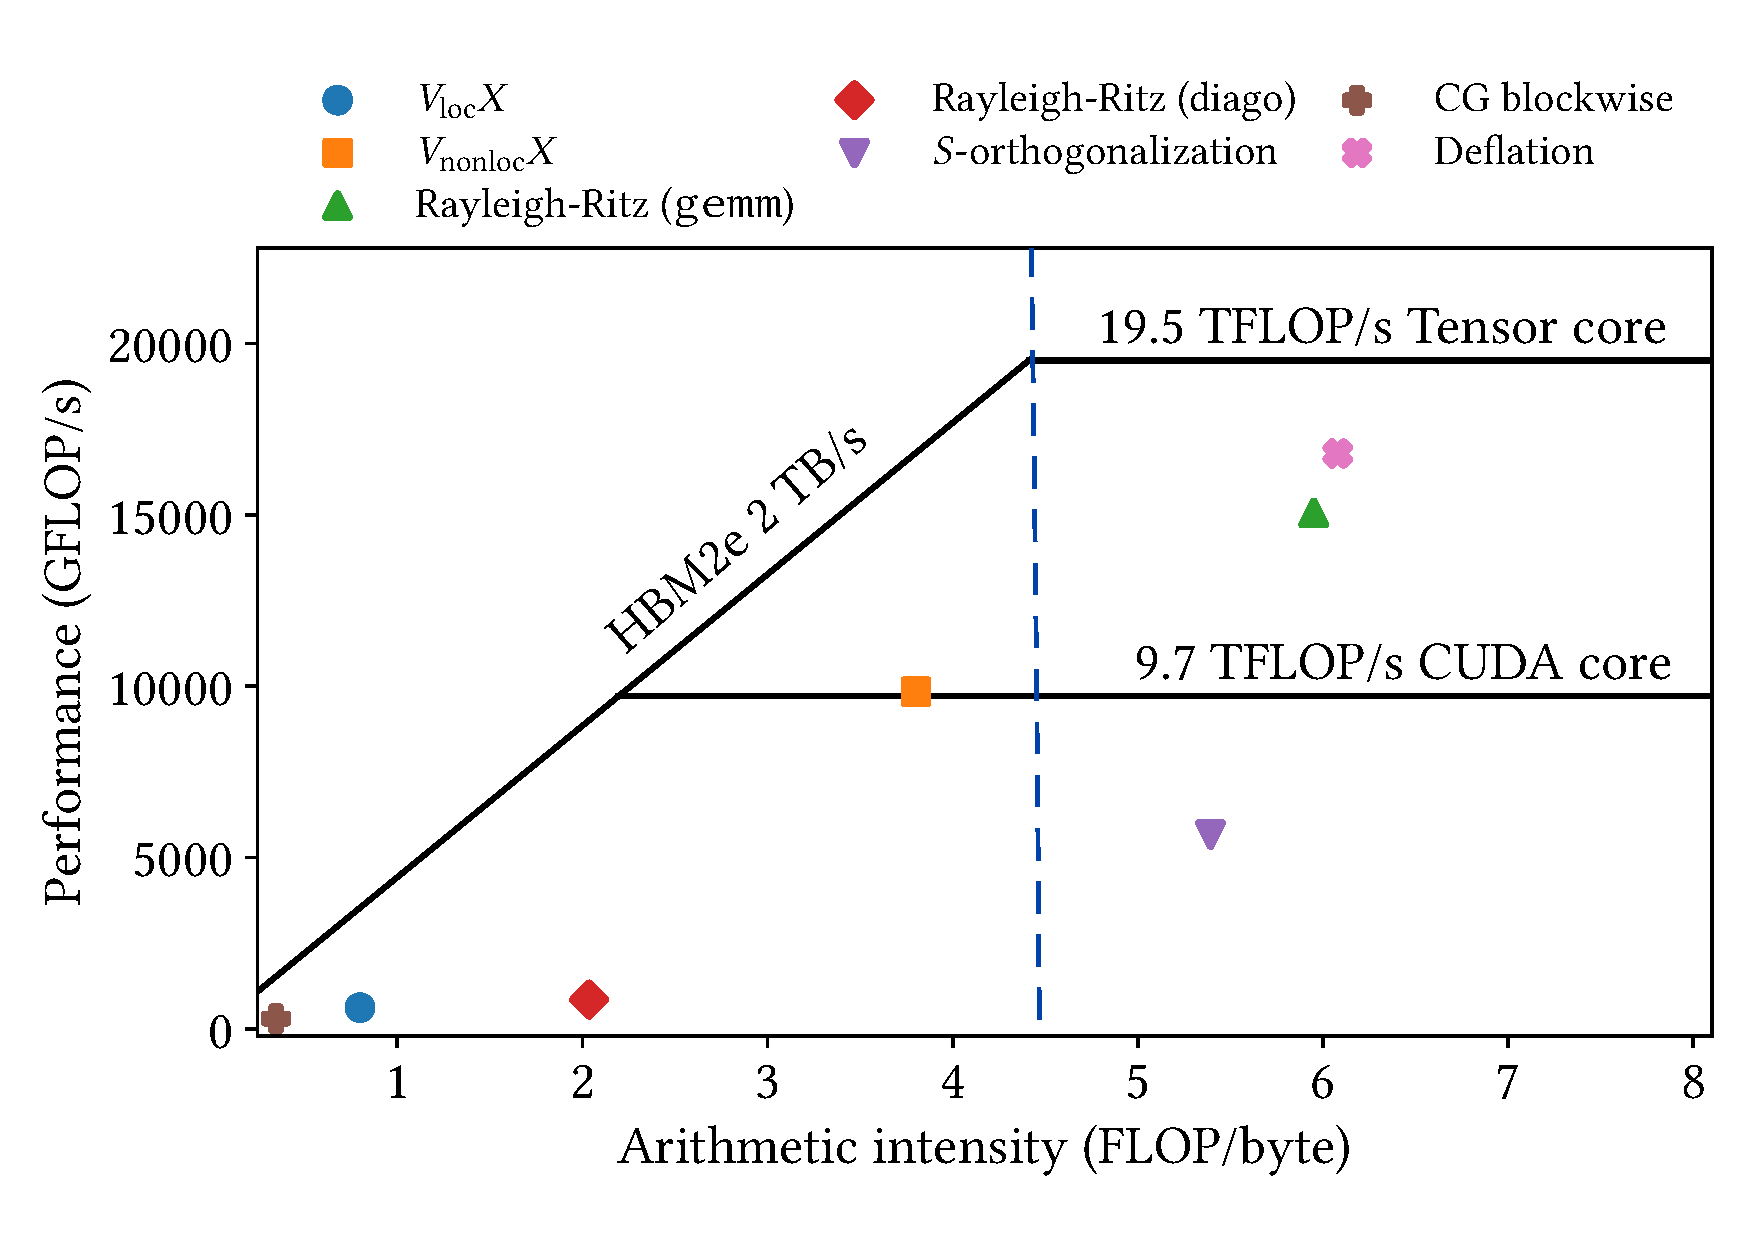
\includegraphics[width=\linewidth]{Figure_5.pdf}
        \subcaption{\lobpcg with 4 blocks.}
        \label{fig:lobpcg4_16mpi}
    \end{minipage}%
    \begin{minipage}{0.48\linewidth}
        \centering
        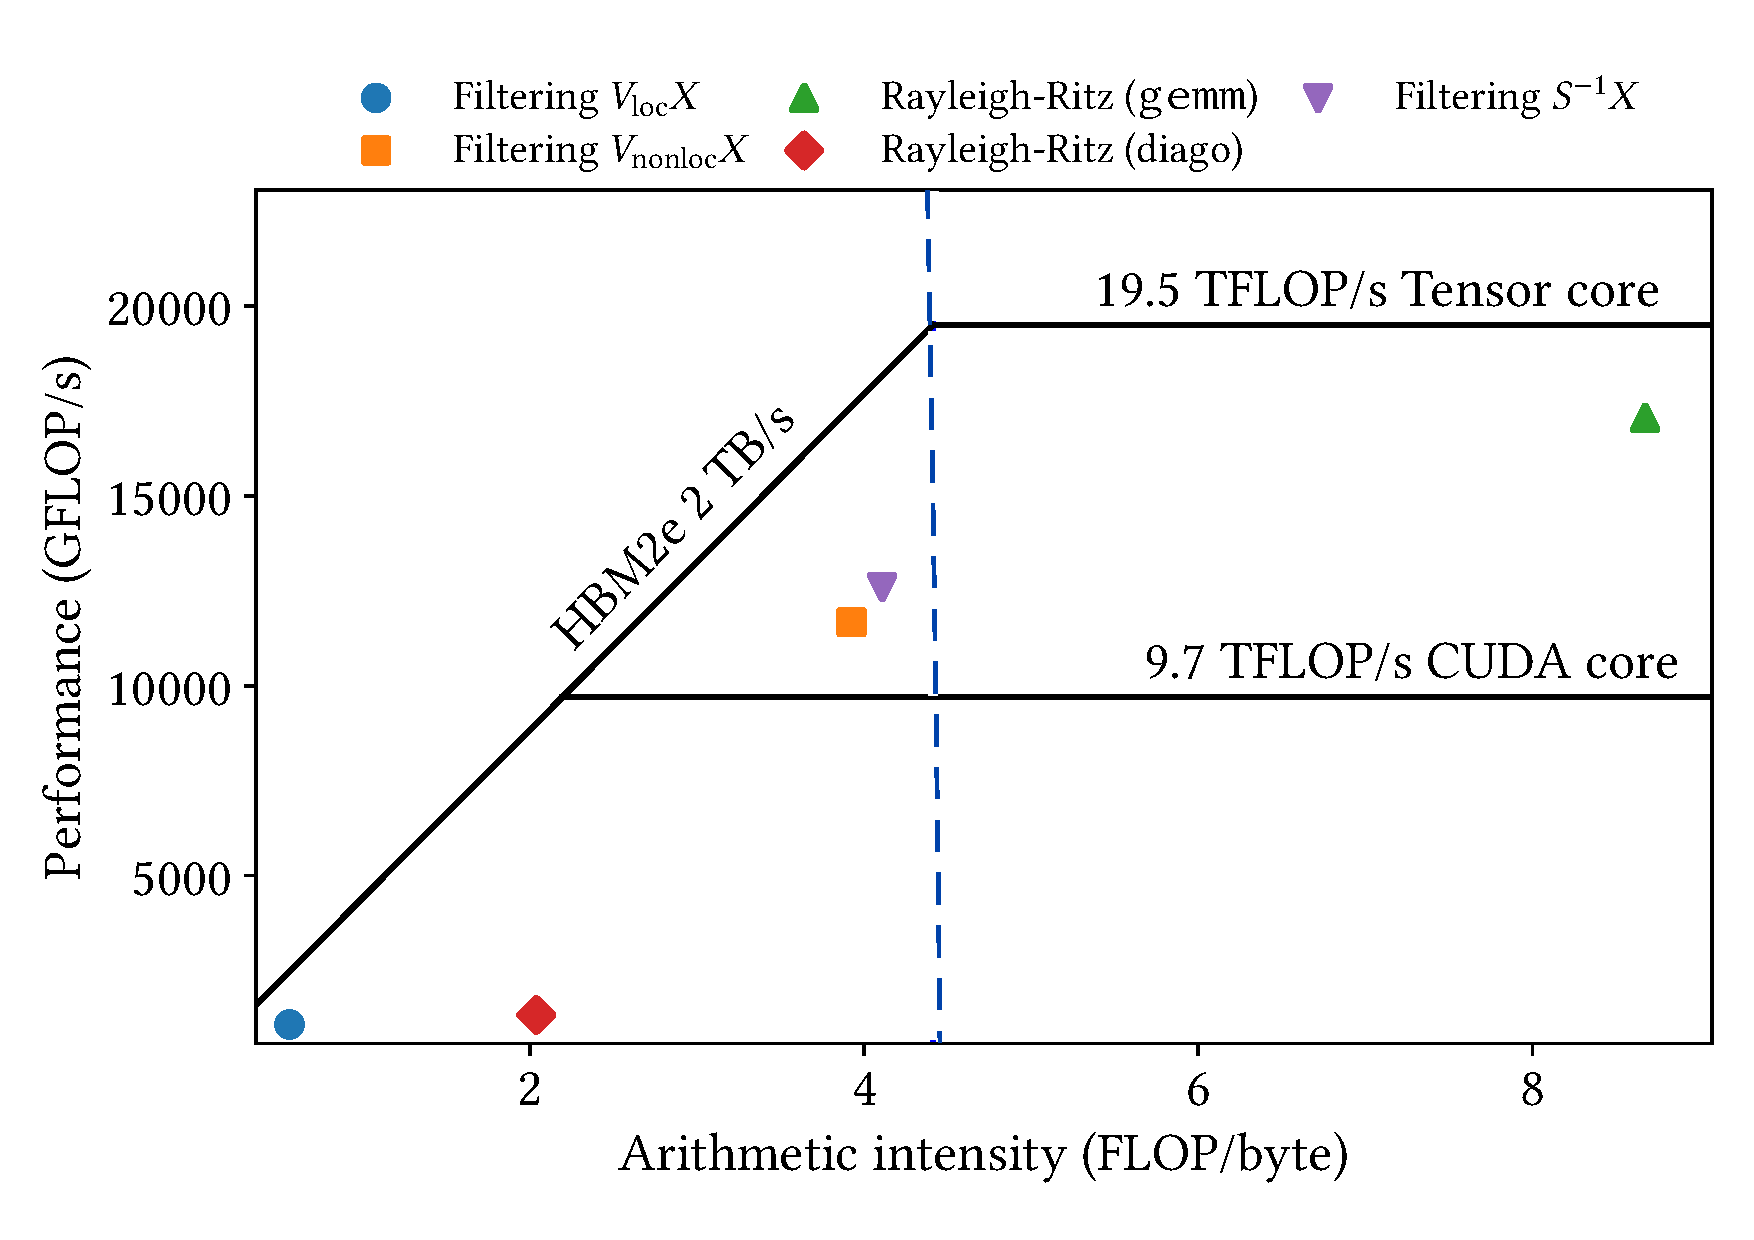
\includegraphics[width=\linewidth]{Figure_6.pdf}
        \subcaption{\chebyshevfiltering.}
        \label{fig:chebfi_16mpi}
    \end{minipage}%
    \hfill
    \caption{Roofline model for (a) the \lobpcg algorithm and (b) the \chebyshevfiltering algorithm, using one \nvidia A100 GPU node (4 GPU devices) for a constant number of Hamiltonian applications (1 SCF step). Key GPU kernels are plotted: (non-)local Hamiltonian–vector products ($V_{\text{(non)loc}}X$), inverse overlap matrix–vector products ($S^{-1}X$), and the Rayleigh-Ritz procedure split into \gemm and diagonalization steps, plus the block-wise conjugate gradient (CG) step and the projection onto the complement of converged blocks (Deflation). The vertical blue dashed line separates the memory-bound region (left) from the compute-bound region (right). The two rooflines represent the peak performance limits of tensor cores (FMA, matrix-matrix multiplications) and \cuda cores, respectively. These benchmarks were performed on the \topaze (CCRT) supercomputer using \nvidia A100 GPUs (see Appendix A). HDM2e stands for high-bandwidth memory 2e. }
    \label{fig:mpi_roofline}
\end{figure*}

Results in Figure~\ref{fig:mpi_roofline} were obtained on one node of \nvidia A100 GPUs (4 \mpi processes, 1 GPU each) and show the performance and arithmetic intensity for process 0, comparing \lobpcg and \chebyshevfiltering algorithms.
We distinguish several components of the Hamiltonian application and iterative diagonalization algorithm. The Hamiltonian application splits into a local part (using FFTs) and a non-local part (using \gemm operations). The Rayleigh-Ritz procedure is further decomposed to \gemm operations and to diagonalization in the trial eigenvector subspace.

The \gemm kernels in both algorithms leverage Tensor cores and are \textit{compute-bound}, confirming their suitability for GPU acceleration. In contrast, the Rayleigh-Ritz solver, implemented through \hegvd linear algebra library calls, is \textit{memory-bound} and \textit{communication-bound}, operating below peak bandwidth. The filtering step reaches peak performance of Tensor cores and is thus \textit{compute-bound}, whereas several kernels fail to attain the memory roof due to data exceeding GPU capacity. To optimize overall performance, an algorithm should minimize both the number of calls and the space dimension of the Rayleigh-Ritz procedure.


From our roofline model benchmarks, the mathematical operations in iterative diagonalization algorithms fall into two categories~\cite{10.1145/1498765.1498785}:
\begin{itemize}
\item \textit{Compute-bound} operations: matrix-free Hamiltonian application and spectral polynomial filtering.
\item \textit{Memory-bound} and \textit{communication-bound} operations: orthogonalization and Rayleigh-Ritz procedure. These operate on relatively small matrices, having all bands and a part of plane waves. Due to their low arithmetic intensity, they do not scale and become a bottleneck.
\end{itemize}

\subsection{Comparison of subspace iteration algorithms}\label{sec:per_gpu_si}

In the previous section, we observed that increasing the number of GPU nodes, while keeping the default parameters of the diagonalization algorithm, is not an effective way to reduce the execution time.
In the following, we examine how adjusting the accuracy of the iterative diagonalization algorithm, specifically by controlling the number of inner iterations, can substantially decrease the runtime. This can be achieved by tuning the block size in the \lobpcg method or the polynomial degree in \chebyshevfiltering. We show that, for the \chebyshevfiltering algorithm, increasing the polynomial degree improves the accuracy of the eigenvectors without degrading overall performance.

For the \lobpcg algorithm, the GPU speed-up at constant number of Hamiltonian applications is defined as $s = T^{\text{CPU}}_{\texttt{nline}} / T^{\text{GPU}}_{\texttt{nline}}$, where $T^{\text{CPU}}_{\texttt{nline}}$ (resp. $T^{\text{GPU}}_{\texttt{nline}}$) denotes the execution time on CPU (resp. GPU) for $\texttt{nline}$ minimization lines—i.e., $\texttt{nline}$ applications of the Hamiltonian operator per eigenvector.
The same indicator applies to the \chebyshevfiltering algorithm: $s = T^{\text{CPU}}_{\texttt{ndeg}} / T^{\text{GPU}}_{\texttt{ndeg}}$, where $T^{\text{CPU}}_{\texttt{ndeg}}$ (resp. $T^{\text{GPU}}_{\texttt{ndeg}}$) is the execution time on CPU (resp. GPU) when using a Chebyshev polynomial of degree $\texttt{ndeg}$.

In Figure~\ref{fig:degree_periter}, we examine the speedup of a single SCF iteration as accuracy increases, by comparing execution times on a single CPU or GPU node. Increasing the number of minimization lines in the \lobpcg algorithm has only a modest effect on speedup, whereas raising the polynomial degree in the \chebyshevfiltering algorithm significantly impacts performance. This indicates that \chebyshevfiltering incurs a lower execution-time penalty when increasing accuracy, compared to \lobpcg. Consequently, \chebyshevfiltering enables faster SCF convergence (fewer steps overall) at less performance cost, making it better suited to GPUs than \lobpcg.

\begin{figure}[t]
    \centering
    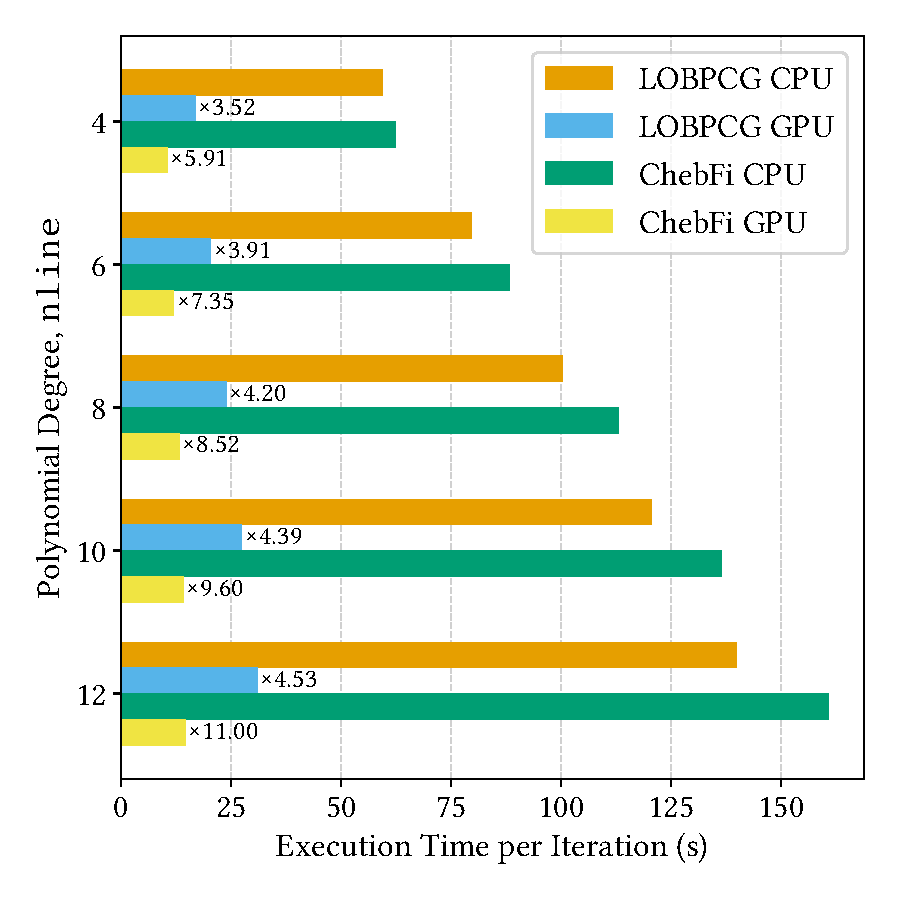
\includegraphics[width=\linewidth]{Figure_7.pdf}
    \caption{Execution times for a single SCF iteration on one CPU or GPU node, as a function of the number of minimization lines (\texttt{nline}) for \lobpcg or the polynomial degree (\texttt{ndeg}) for \chebyshevfiltering (abbreviated as ChebFi). The numbers next to the histograms indicate the CPU/GPU speedup at constant number of Hamiltonian applications, as defined in Section~\ref{sec:per_gpu_si}. These benchmarks were performed on the \topaze (CCRT) supercomputer using \amd Milan processors and \nvidia A100 GPUs (see Appendix~\ref{sec:gpu_specifs}).}
    \label{fig:degree_periter}
\end{figure}

Table~\ref{tab:chebfi_lobpcg_perf} shows that the accuracy gains from \chebyshevfiltering also reduce the final number of self-consistent field (SCF) iterations required for convergence.
In \lobpcg, the number of SCF iterations is already minimal even with few minimization lines, as the eigenvectors—particularly the last ones—are well converged. Thus, increasing the number of lines adds unnecessary computational workload without reducing SCF iterations further.
In contrast, raising the polynomial degree in \chebyshevfiltering substantially improves eigenvector convergence and thereby decreases the number of SCF iterations. Like \lobpcg, there is a minimal number of SCF iterations beyond which no further precision is gained, while computation time continues to rise with the polynomial degree. \chebyshevfiltering thus offers an optimal polynomial degree that maximizes GPU acceleration, though this critical value likely depends strongly on the simulated material.

\begin{table}[t]
\centering
\begin{tabular}{lcccc}
\hline
Algorithm & Degree & Wall Time & \# SCF & Squared WF residual  \\ %& Per-iteration time
          & \texttt{ndeg} &   (s)        &  iterations & at iter. 1 \\ %& (s/iter)
\hline
\multirow{6}{*}{ChebFi}
  & 4  & 295.8 & 28 &  3.0e-6 \\
  & 6  & 204.0 & 17 &  2.6e-6 \\
  & 8  & 198.8 & 15 &  1.5e-6 \\
  & 10 & 198.8 & 14 &  1.0e-6 \\
  & 12 & 204.7 & 14 &  8.0e-7 \\
  & 14 & 221.4 & 14 &  2.5e-7 \\
\hline
Algorithm & \texttt{nline} & Wall Time & \# SCF & Squared WF residual \\ %& Per-iteration time
          &  &     (s)      &  iterations & at iter. 1 \\ %& (s/iter)
\hline
\multirow{5}{*}{\lobpcg}
  & 4  & 236.3 & \multirow{5}{*}{14} & 2.0e-7 \\
  & 6  & 285.6 &  &  3.5e-9 \\
  & 8  & 334.6 &  &  2.5e-10 \\
  & 10 & 384.4 &  &  2.5e-10 \\
  & 12 & 432.6 &  &  2.5e-10 \\
\hline
\end{tabular}
\caption{Execution times and number of SCF iterations in \abinit{} on a single GPU node, for ground-state determination of the energy, forces, and stress tensor in a 320-atom \ce{Ga2O3} crystal (1536 electronic bands). Results are shown as a function of the number of minimization lines (\texttt{nline}) for \lobpcg or the polynomial degree (\texttt{ndeg}) for \chebyshevfiltering (abbreviated as ChebFi). All runs used the same stopping criterion based on the density residual, with \lobpcg employing a fixed number of 4 blocks. Last column shows the maximum value of the squared wave function residual $|H\Psi_{nk} - \epsilon_{nk}S\Psi_{nk}|^2$ at the end of the first SCF iteration
These benchmarks were performed on the \topaze (CCRT) supercomputer using 4 \nvidia A100 GPUs (see Appendix~\ref{sec:gpu_specifs}).}
\label{tab:chebfi_lobpcg_perf}
\end{table}

One major limitation of the \chebyshevfiltering algorithm on CPUs is that the accuracy gains from increasing the polynomial degree fail to offset the filtering overhead per inner iteration. This leads to an overall slowdown in the self-consistent field (SCF) cycle execution time, despite fewer iterations.
In contrast, on GPUs, Table~\ref{tab:chebfi_lobpcg_perf} shows that raising the polynomial degree pays off due to highly accelerated Hamiltonian applications. The inner iterations then outperform even the best-case \lobpcg scenario, without significant accuracy loss. The last column of the table shows that LOBPCG achieves much higher accuracy at first inner iteration, without lowering the number of outer SCF iterations. \chebyshevfiltering also provides finer control, offering more flexibility to balance accuracy and speed by gradually tuning the degree as needed.

\section{Conclusion and perspectives}

In this paper, we demonstrate that the GPU port of the \abinit software package enables highly efficient plane-wave density functional theory calculations. This GPU port was first made available in \abinit v10.0 and has been further improved and expanded in later versions. The complete GPU port we present in this paper is production-ready in \abinit v10.6 or later. Performance is excellent on \nvidia GPUs from the Ampere and Hopper families, as well as on \amd MI-series GPUs, though it requires graphics accelerators with high double-precision computing capabilities.
A simple porting effort alone does not ensure high performance; algorithmic adaptations are essential to make diagonalization procedures more GPU-optimized. Iterative diagonalization algorithms must be revisited to prioritize compute-bound operations with high arithmetic intensity, such as applying the Hamiltonian operator to large batches of wave functions.
In this regard, spectrum polynomial filtering algorithms, such as \chebyshevfiltering, are the most suitable, as they build the eigenvector subspace through repeated Hamiltonian applications on extensive trial vector sets. In contrast, the \lobpcg algorithm, which relies on block-wise orthogonalization via parallel conjugate gradients, remains more memory-bound.
Memory-bound operations like subspace orthogonalization also limit multi-GPU scaling. Theoretical cost models and \abinit benchmarks both confirm that matrix-matrix multiplications on large wave-function sets boost arithmetic intensity and should thus be favored. On the other hand, the Rayleigh-Ritz procedure, involving orthogonalization, should be performed as rarely as possible, on the smallest eigenvector subspace.

To reduce the impact of compute-bound subspace diagonalization, a viable solution proposed in the literature is the Spectrum Slicing method \cite{LIOU2020107330,SCHOFIELD2012497}. This approach enables fast eigensolutions for large batches of Hermitian matrices processed in parallel on GPUs, while substantially reducing the size of the Rayleigh-Ritz operation.
This method would facilitates simulations of larger systems by distributing wave functions across GPUs during Rayleigh-Ritz steps. It avoids a global Rayleigh-Ritz procedure across all bands, instead computing smaller independent eigenvalue slices. In such polynomial filter-based methods, the polynomial degree must be much higher than in standard \chebyshevfiltering. As demonstrated in this paper, the numerous Hamiltonian applications involved likely have only limited overhead on GPUs.


\section*{Acknowledgments}

This project was provided with computing HPC and storage resources by GENCI at CINES and IDRIS computing centers thanks to the grant 2023-AD010914563 on the supercomputers \jeanzay and \adastra.
Part of the work was performed using HPC resources from CCRT (CEA, France) on the \topaze supercomputer.
This project was partly supported by the European Union’s Horizon 2020 research and innovation program under the grant agreement N° 951786 (NOMAD CoE).
The authors are grateful to Cl\'ementine Barat for insightful discussions regarding \chebyshevfiltering algorithm.

\bibliographystyle{unsrt}
\bibliographystyle{cpc}
\bibliography{bibliography}

\appendix

\section{Machine specifications} \label{sec:gpu_specifs}

Technical specifications of the CPU/GPU hybrid partitions used for benchmarking are shown in Table~\ref{tab:gpu_specifs}.

\begin{table*}[t]
    \centering
    \begin{tabular}{l|c|c|c}\toprule
          Supercomputer          & \topaze & \jeanzay & \adastra  \\ \midrule
          Center                 & CCRT (France)~\cite{CCRT2026} & IDRIS (France)~\cite{IDRIS2026} & CINES (France)~\cite{CINES2026}  \\
          Model                  & BullSequana XH2000 & HPE SGI 8600 & HPE Cray EX4000 \\
          \# Nodes               & 75 & 364 & 356 \\
          Processors per node    & 2 \amd EPYC Milan 7763 & 2 Intel Xeon Platinum 8468 & \amd EPYC Trento (3e gen.) \\
          CPU frequency          &  2,45 GHz    & 2,10 GHz & 2,40 GHz \\
          GPUs per node          & 4 \nvidia A100 SXM4 & 4 \nvidia H100 SXM5 & 4 \amd Instinct MI250X \\
          GPU memory bandwidth   & 2 TB/s & 3 TB/s & 3.2 TB/s \\
          Memory per GPU         & 80 GB & 80 GB & 128 GB \\
          \# Cores per node      & 128 & 96 & 64 \\
          RAM per node           & 512 GB & 512 GB & 256 GB \\
          Peak performance       & 4,3 PFlop/s & 126 PFlop/s & 74 PFlop/s \\
          Power consumption      &      & 1400 kW & 921.48 kW \\
          Network model          & InfiniBand HDR & InfiniBand NDR & Slingshot-11 \\
          Network bandwidth      & 200 Gbit/s & 400 Gbit/s & 100 Gbit/s \\ \bottomrule
    \end{tabular}
    \caption{Technical specifications of the hybrid (CPU/GPU) partitions of the 3 supercomputers used in the present article.}
    \label{tab:gpu_specifs}
\end{table*}

\vspace{1em}

\section{\abinit GPU-enabled functionalities} \label{sec:gpu_features}

Table~\ref{tab:gpu_features} summarizes GPU-enabled functionalities in \abinit version 10.6.

\begin{table*}[b]
    \centering
    \begin{tabular}{c|l}\toprule
          Topic & Property or method \\ \midrule
          \multirow{7}{*}{Ground-state properties (DFT)}  & Total energy \\
          & Forces, stress tensor \\
          & Hybrid functionals \\
          & DFT+U \\
          & \lobpcg algorithm \\
          & \chebyshevfiltering algorithm \\ \hline
          \multirow{6}{*}{Response functions (DFPT)} & 
          Response to perturbation of \kpoint  \\
          & Response to perturbation of electric field \\
          & Atomic vibrations (phonons at $q=0$) \\
          & Atomic vibrations (phonons at $q\neq 0$) \\ 
          & Elastic tensor \\
          & Metals \\ \hline
          \multirow{3}{*}{Many-body theory (DMFT) } & Green function computation \\
          & Hubbard-I solver \\
          & CT-QMC solver (partially ported) \\
          \bottomrule
    \end{tabular}
    \caption{\abinit functionalities ported to GPU as of version 10.6 grouped by physical property. All listed features are implemented in the following formalisms: norm-conserving pseudopotentials, projector augmented-wave approach (PAW), collinear and non-collinear magnetism, spin-orbit coupling.}
    \label{tab:gpu_features}
\end{table*}

\end{document}
